%
% flowcharts.tex
%
% Copyright (C) 2019 by Gabriel Mariano Marcelino <gabriel.mm8@gmail.com>.
%
% Relatório 3 do Trabalho Final da Disciplina EEL510265.
%
% This work is licensed under the Creative Commons Attribution-ShareAlike 4.0
% International License. To view a copy of this license,
% visit http://creativecommons.org/licenses/by-sa/4.0/.
%

%
% \brief Flowcharts section.
%
% \author Gabriel Mariano Marcelino <gabriel.mm8@gmail.com>
%
% \version 0.1.0
%
% \date 21/11/2019
%

\section{Fluxogramas} \label{sec:flowcharts}

Os principais fluxogramas do sistema são apresentados a seguir.

\subsection{Geral}

O fluxograma geral de execução do sistema pode ser visto na \autoref{fig:flowchart-general}.

\begin{figure}[!ht]
    \begin{center}
        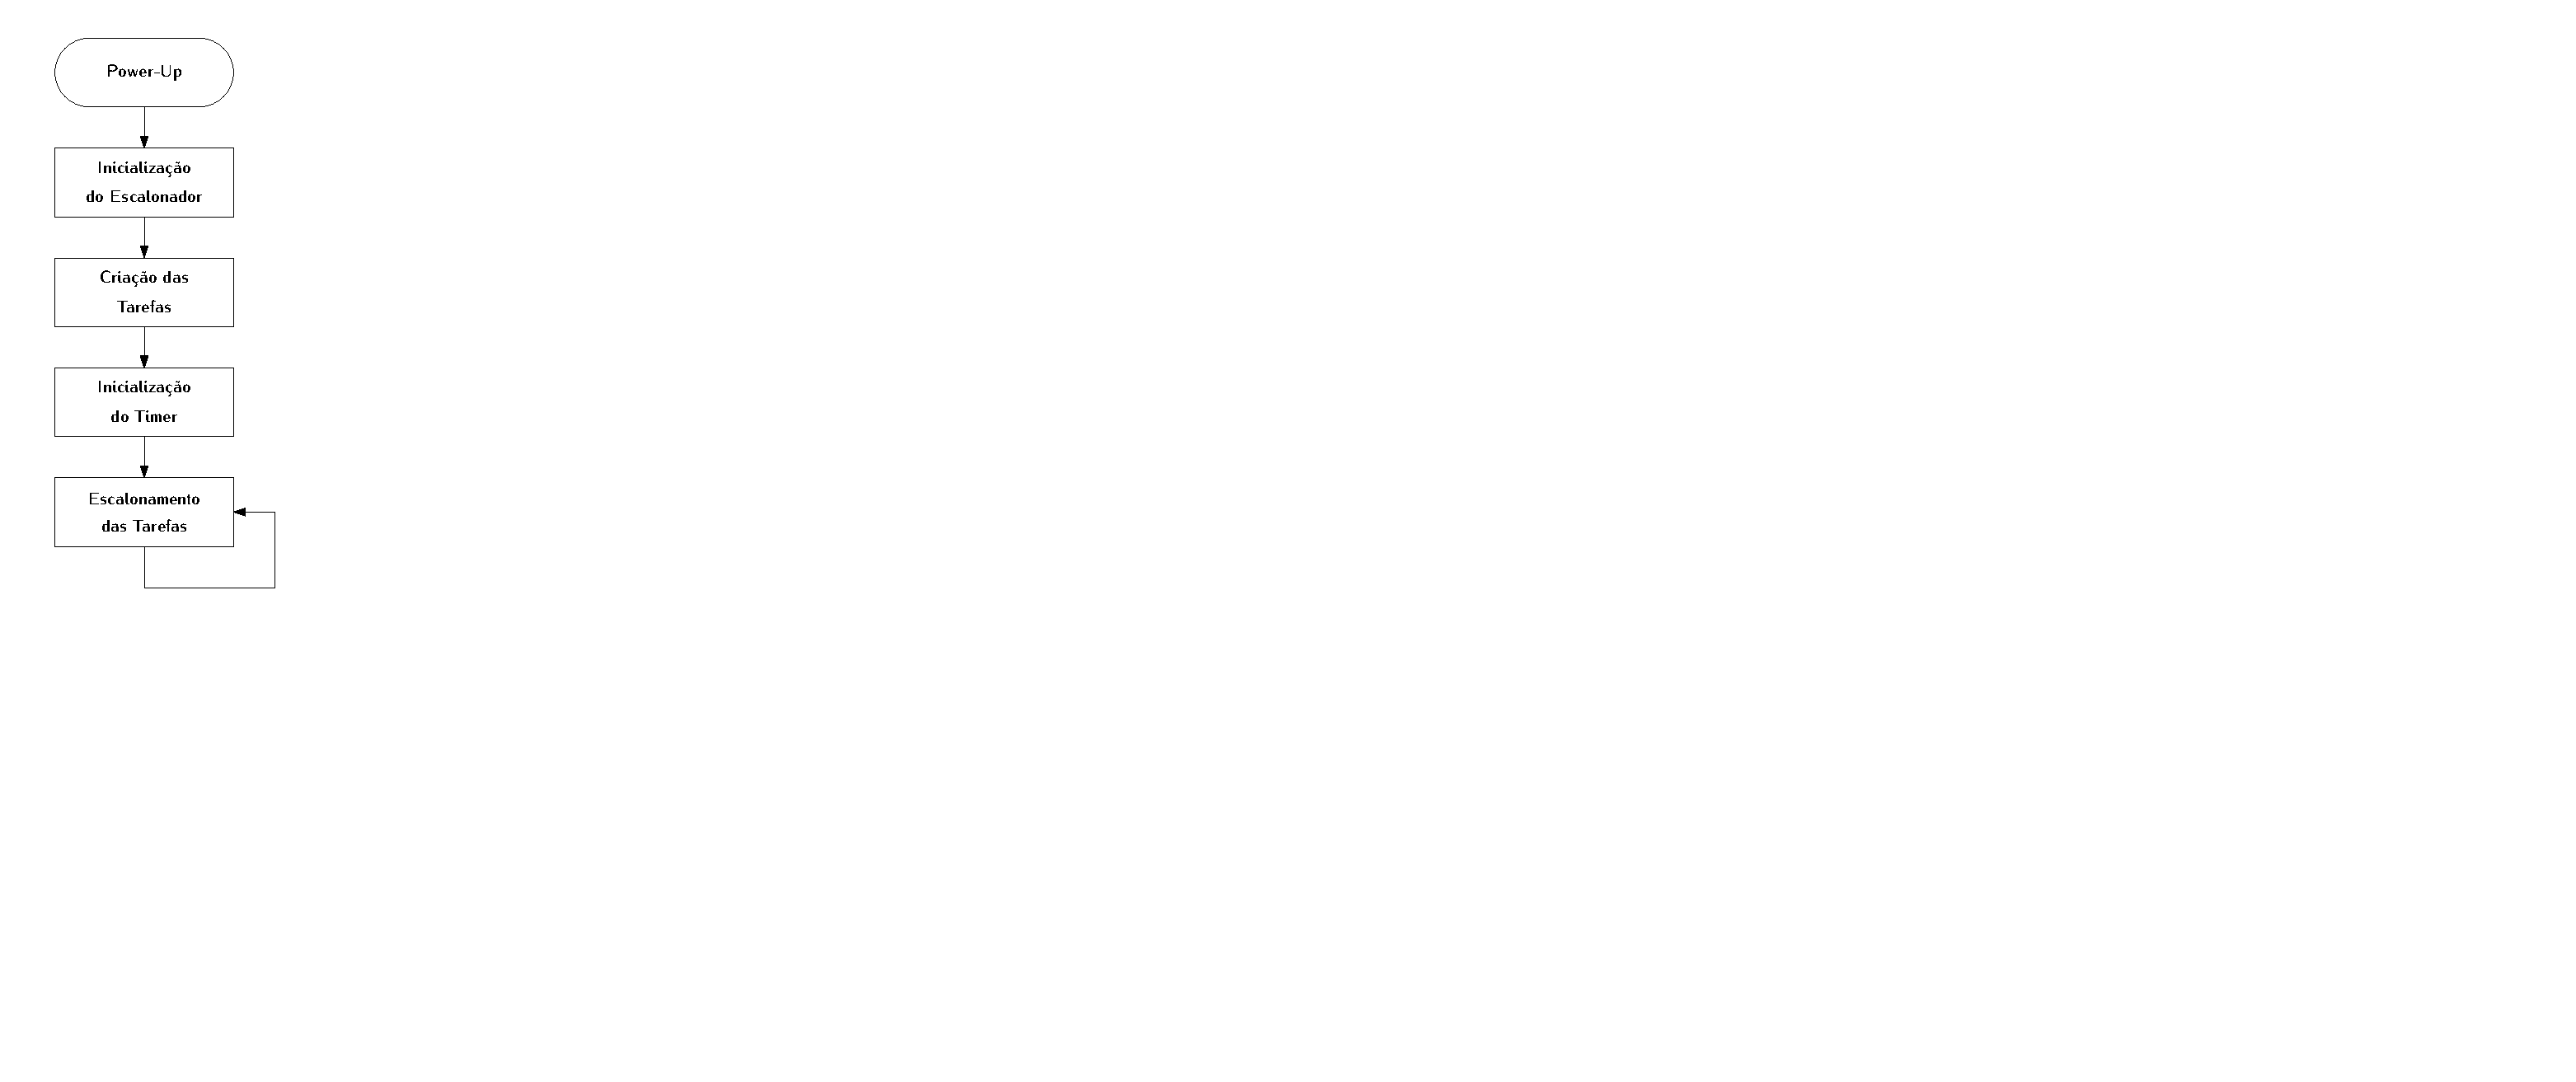
\includegraphics[width=0.3\textwidth]{figures/flowchart_general.pdf}
        \caption{Fluxograma geral do sistema.}
        \label{fig:flowchart-general}
    \end{center}
\end{figure}

\subsection{Interrupção do Timer}

O fluxograma de execução da interrupção do \textit{timer} do sistema (utilizado para o controle de tempo do escalonador) pode ser visto na \autoref{fig:flowchart-timer}.

\begin{figure}[!ht]
    \begin{center}
        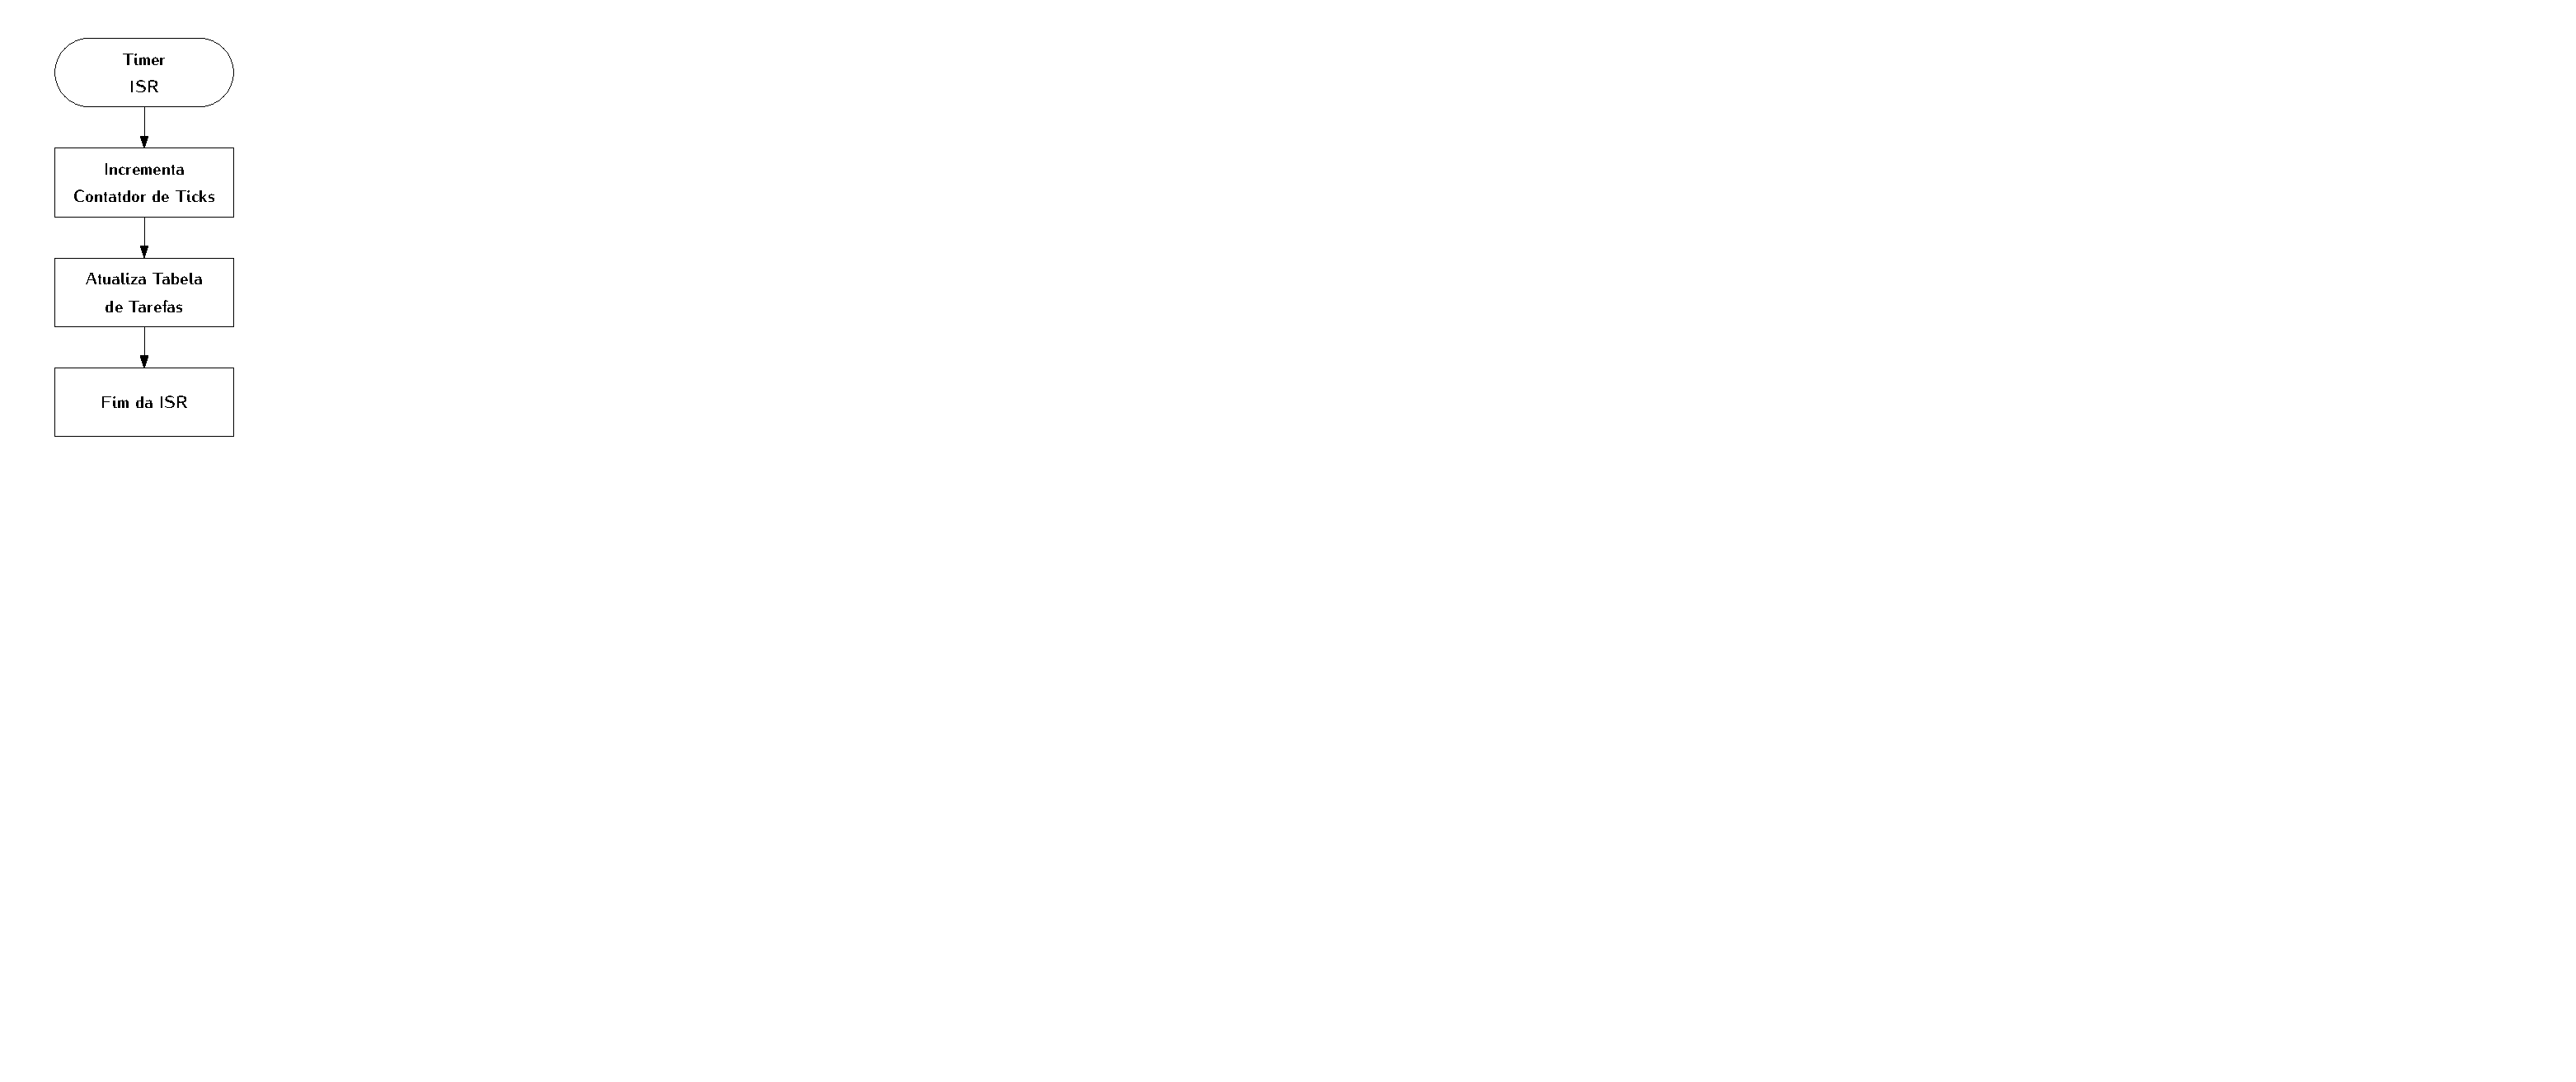
\includegraphics[width=0.25\textwidth]{figures/flowchart_timer.pdf}
        \caption{Fluxograma da interrupção do \textit{timer} do sistema.}
        \label{fig:flowchart-timer}
    \end{center}
\end{figure}

Neste diagrama, considera-se a implementação da máquina de vendas em um microcontrolador embarcado. Para a versão de desenvolvimento, que é executada em um microcomputador, deve-se acrescentar uma rotina de espera (\textit{sleep}) ao fluxo de execução. Neste, a caso a rotina de espera simula o comportamento da rotina de interruoção (ISR) do \textit{timer}.
